\def\retinafocusidea{
    Lấy cảm hứng từ hai mô hình RetinaFace \cite{deng2020retinaface} và AutoFocus \cite{najibi2019autofocus}, mô hình RetinaFocus được xây dựng nhằm tận dụng điểm mạnh và khắc phục điểm yếu của cả hai mô hình trên trong một mô hình duy nhất, từ đó, giải quyết tốt bài toán nhận diện khuôn mặt trong ảnh chất lượng cao.

    \noindent
    Mô hình RetinaFace \cite{deng2020retinaface} đạt độ chính xác tương đối cao trên bộ dữ liệu WIDER FACE cùng với tốc độ xử lý đạt mức chấp nhận được trên bài toán nhận diện khuôn mặt.
    Mặc dù sử dụng FPN trong kiến trúc mô hình xương sống của mình, mô hình RetinaFace \cite{deng2020retinaface} vẫn chưa thể dự đoán với vị trí hộp giới hạn\index{hộp giới hạn} chính xác và với độ tự tin cao hết những mặt có kích thước nhỏ.
    Do đó, khi xử lý ảnh có kích thước lớn, để duy trì được độ chính xác cao, nhóm tác giả vẫn sử dụng chiến lược Image Pyramids và điều đó khiến cho tốc độ xử lý của RetinaFace \cite{deng2020retinaface} tăng lên nhiều lần. \\
    Bên cạnh đó, mô hình AutoFocus \cite{najibi2019autofocus}, lại là một giải pháp rất thông minh để xử lý ảnh với chiến lược Image Pyramids nhưng với tốc độ cao và chi phí tính toán thấp. \\
    Từ những điểm yếu của mô hình RetinaFace \cite{deng2020retinaface} khi xử lý ảnh chất lượng cao và những điểm mạnh của mô hình AutoFocus \cite{najibi2019autofocus}, chúng tôi đề xuất mô hình RetinaFocus giải bài toán nhận diện khuôn mặt trong ảnh chất lượng cao với độ chính xác tương đương và cải thiện đáng kể tốc độ tính toán.

    \noindent
    Mô hình RetinaFocus gồm hai nhánh: nhánh xác định đối tượng\index{nhánh xác định đối tượng} và nhánh tập trung đối tượng\index{nhánh tập trung đối tượng}. \\
    - Nhánh xác định đối tượng\index{nhánh xác định đối tượng} là một mô hình nhận diện khuôn mặt với nhiệm vụ đưa ra kết quả về vị trí của khuôn mặt trên ảnh.
    Trong mô hình RetinaFocus, nhánh xác định đối tượng\index{nhánh xác định đối tượng} được xây dựng dựa trên mô hình RetinaFace \cite{deng2020retinaface}. \\
    - Nhánh tập trung đối tượng\index{nhánh tập trung đối tượng} là một mô hình Conv với nhiệm vụ đưa ra dự đoán giúp xác định được các khu vực đáng chú ý trên ảnh và loại bỏ các khu vực khả năng cao không chứa khuôn mặt, các khu vực có khả năng chứa khuôn mặt sau đó sẽ được zoom in, crop và đưa vào cả nhánh xác định đối tượng\index{nhánh xác định đối tượng} và nhánh tập trung đối tượng\index{nhánh tập trung đối tượng}.
    Trong mô hình RetinaFocus, nhánh tập trung đối tượng\index{nhánh tập trung đối tượng} được xây dựng dựa trên mô hình AutoFocus \cite{najibi2019autofocus}.

    \begin{figure}[H]
        \centering
        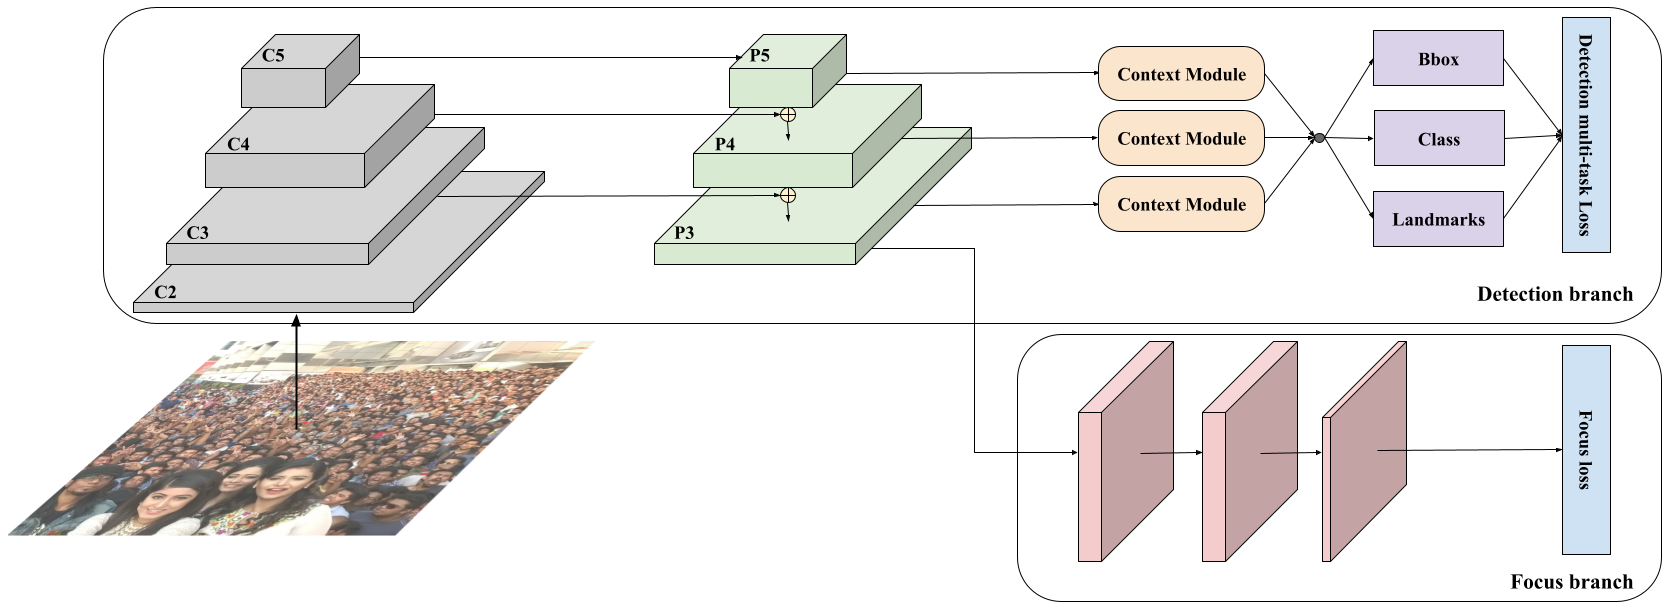
\includegraphics[width=15cm] {images/retinafocus_architecture}
        \caption{Kiến trúc của mô hình RetinaFocus.}
        \label{fig:retinafocus_architecture}
    \end{figure}

    \noindent
    Hình trên là một ví dụ về kiến trúc mô hình RetinaFocus khi sử dụng bản đồ đặc trưng\index{bản đồ đặc trưng} $P_3$ của FPN làm đầu vào cho Nhánh tập trung đối tượng\index{nhánh tập trung đối tượng}.
    Các bản đồ đặc trưng\index{bản đồ đặc trưng} khác của FPN cũng đều có thể được sử dụng làm đầu vào cho Nhánh tập trung đối tượng\index{nhánh tập trung đối tượng}.
}